%%%%	Tim Petty --- Mozgalo 2019.

% Klasa dokumenta: scrartcl.
\documentclass[paper = a4, fontsize = 11pt, DIV = 12, BCOR = 0pt, headings = standardclasses, numbers = endperiod]{scrartcl}

% Neke opcije za "kvalitetniji" (barem u smislu eksportiranja teksta) PDF dokument.
\pdfinterwordspaceon
\input{glyphtounicode}
\pdfgentounicode=1

% Paket za geometrijsko uredenje stranica.
\usepackage[margin = 25mm]{geometry}

% Paket za uredenje izgleda stranica.
\usepackage{scrlayer-scrpage}

% (Uglavnom) matematicki paketi (dodatno: tikz + pgfplots + pgfplotstable za generiranje grafova, lstlistings za programske kodove, siunitx za SI i srodne mjerne jedinice, units za mjerne jedinice opcenito).
\usepackage{amsbsy}
\usepackage{amsmath}
\usepackage{amssymb}
\usepackage{amstext}
\usepackage{amsthm}
%\usepackage{bm}
%\usepackage{bbm}
\usepackage{listings}
\usepackage{mathtools}
\usepackage{numprint}
\usepackage{pgfplots}
\usepackage{pgfplotstable}
\usepackage[binary-units = true, output-decimal-marker = {{,}}]{siunitx}
\usepackage{stackrel}
\usepackage{thmtools}
\usepackage{tikz}
\usepackage{units}

% Paketi za odabir familije fontova, dobro procesuiranje i prikazivanje teksta i za jezik.
\usepackage{lmodern}
\usepackage{txfonts}
\usepackage{newtxtext}
\usepackage{newtxmath}
\usepackage[T1]{fontenc}
\usepackage[utf8]{inputenc}
\usepackage[final]{microtype}
\usepackage[croatian]{babel}

% Indeks, pojmovnik i bibliografija.
\usepackage[xindy]{imakeidx}
\usepackage[xindy]{glossaries}
\usepackage[backend = biber, indexing = true, sorting = nyvt, style = numeric, bibstyle = numeric, citestyle = numeric-comp, sortcites = true]{biblatex}
\usepackage[nottoc]{tocbibind}
\usepackage{xpatch}

% Reference i hiperlinkovi.
\usepackage{varioref}
\usepackage[unicode = true]{hyperref}
\usepackage{cleveref}
\usepackage{bookmark}
\usepackage{url}

% Postavke PDF dokumenta pomocu paketa hyperref.
\hypersetup{
	pdfstartview = ,
	pdftitle = {Dokumentacija za predaju rješenja u sklopu natjecanja Mozgalo},
	pdfsubject = {Mozaglo 2019.},
	pdfauthor = {Natjecateljski tim},
	pdfkeywords = {Mozgalo, data-mining, klasifikacija, binarna klasifikacija, strojno učenje, Python, CatBoost, hiperparametarska optimizacija}
}

% Paket za uredenje enumeriranja jednadzbi, tablica, slika i slicnih objekata.
\usepackage{chngcntr}

% Kompatibilnost paketa PGFPlots.
\pgfplotsset{compat = 1.15}

% Dodatni paketi.
\usepackage{array}
\usepackage{caption}
\usepackage{csquotes}
\usepackage{graphicx}
\usepackage{subcaption}
\usepackage{multicol}
\usepackage{multirow}
\usepackage{tabularx}
\usepackage{xcolor}
\usepackage{url}

% Paket za prikaz rubova dijelova stranica (zaglavlje, glavni dio, podnozje).
%\usepackage{showframe}

% Paket za generiranje "lorem ipsum" teksta.
\usepackage{lipsum}

% Definiranje navodnih znakova.
\MakeOuterQuote{"}

% Indeks.
\makeindex

% Pojmovnik.
\makeglossaries

% Literatura.
%\addbibresource{bibliography.bib}

% Definicije okruzenja za definicije, teoreme, leme, propozicije, korolare, slutnje, napomene i primjere. Svako okruzenje ima normalnu definiciju (na primjer, \begin{definition}...\end{definition}) koja rezultira enumeriranim okruzenjem, i definiciju s asteriskom (na primjer, \begin{definition*}...\end{definicition*}) koja rezultira ne-enumeriranim okruzenjem.
\declaretheorem[style = definition, numberwithin = section, name = {Definicija}]{definition}
\declaretheorem[style = definition, numbered = no, name = {Definicija}]{definition*}
\declaretheorem[style = plain, sibling = definition, name = {Teorem}]{theorem}
\declaretheorem[style = plain, numbered = no, name = {Teorem}]{theorem*}
\declaretheorem[style = plain, sibling = definition, name = {Lema}]{lemma}
\declaretheorem[style = plain, numbered = no, name = {Lema}]{lemma*}
\declaretheorem[style = plain, sibling = definition, name = {Propozicija}]{proposition}
\declaretheorem[style = plain, numbered = no, name = {Propozicija}]{proposition*}
\declaretheorem[style = plain, sibling = definition, name = {Korolar}]{corollary}
\declaretheorem[style = plain, numbered = no, name = {Korolar}]{corollary*}
\declaretheorem[style = plain, sibling = definition, name = {Slutnja}]{conjunction}
\declaretheorem[style = plain, numbered = no, name = {Slutnja}]{conjunction*}
\declaretheorem[style = remark, sibling = definition, name = {Napomena}]{remark}
\declaretheorem[style = remark, numbered = no, name = {Napomena}]{remark*}
\declaretheorem[style = remark, sibling = definition, name = {Primjer}, qed = {\ensuremath{{\lhd}}}]{example}
\declaretheorem[style = remark, numbered = no, name = {Primjer}, qed = {\ensuremath{{\lhd}}}]{example*}

% Definicije naredbi za skupove.
\newcommand*{\naturals}{\mathbb{N}}
\newcommand*{\integers}{\mathbb{Z}}
\newcommand*{\rationals}{\mathbb{Q}}
\newcommand*{\reals}{\mathbb{R}}
\newcommand*{\complex}{\mathbb{C}}

% Definicija naredbe za skupove matrica.
\newcommand*{\matrices}[2]{\mathrm{M}_{#1} \left( #2 \right)}

% Definicije naredbi za kovarijancu i vektorizaciju.
\DeclareMathOperator{\cov}{cov}
\DeclareMathOperator{\vecmatrix}{vec}

% Definicije naredbi za koristenu statisticku notaciju.
\newcommand*{\column}[1]{\mathbbm{#1}}
\newcommand*{\colvector}[1]{\bm{#1}}
\newcommand*{\transponent}{\mathsf{T}}
\newcommand*{\sample}[1]{\mathbbm{#1}}
\newcommand*{\mean}[1]{\bar{#1}}

% Definiranje "lijepog" stila programskih kodova.
\lstdefinestyle{lijepo}
{
	breaklines = true,
	breakatwhitespace = true,
	numbers = left,
	stepnumber = 1,
	numberstyle = {\footnotesize \ttfamily \bfseries},
	tabsize = 4,
	frame = none,
	basicstyle = {\footnotesize \ttfamily},
	stringstyle = {\color{red}},
	keywordstyle = {\bfseries \color{blue}},
	commentstyle = {\itshape \color{gray}},
	showstringspaces = true
}


% Naslov, podnaslov, autor i datum.
\title{Dokumentacija za predaju rješenja u sklopu natjecanja \emph{Mozgalo}}
\subtitle{\emph{Mozgalo} 2019.}
\author{Natjecateljski tim}
\date{Svibanj 2019.}

% Postavljanje stila stranica na scrheadings.
\pagestyle{scrheadings}

\begin{document}
	\maketitle

	\section{Opis odabranog pristupa za rješavanje problema}
	\label{sec:opis_pristupa}

	Zadatak ovogodišnjeg natjecanja \href{http://estudent.hr/category/natjecanja/mozgalo/}{\emph{Mozgalo}} bio je predviđanje ponašanja klijenata banke \href{http://rba.hr/}{\emph{Reiffeisenbank Hrvatska}}: predvidjeti hoće li se ugovor o kreditu odnosno depozitu raskinuti prije ugovorenog datuma ili ne. Taj se problem može shvatiti kao binarna klasifikacija ugovora.

	\par

	Autori ovog rješenja klasifikaciji ugovora pristupili su stablima odlučivanja. Rješenje je razvijeno u \href{http://python.org}{programskom jeziku \emph{Python}} (inačica 3.X.X) \href{http://catboost.ai}{paketom \emph{CatBoost}} (inačica 0.14.2) i sastoji se od simetričnih stabala odlučivanja, za koja implementacija \href{http://catboost.ai}{\emph{CatBoost}-a} omogućuje dohvaćanje značajnosti značajki. To je svojstvo bilo poželjno zbog interpretabilnosti rješenja.

	\par

	Osim \href{http://docs.python.org/3/library/}{standardne biblioteke \emph{Pythona}} i \href{http://catboost.ai/docs}{biblioteke paketa \emph{CatBoost}-a}, korištene su biblioteke \href{http://scipy.org/docs.html}{\emph{SciPy} paketa} i \href{http://hyperopt.github.io/hyperopt/}{paket \emph{hyperopt}}. Konačni je k\^{o}d, naravno, ipak vlastiti rukopis.

	\par

	\section{Opis \emph{dataseta}}
	\label{sec:opis_dataseta}

	Osim konstrukcije samog klasifikacijskog modela, veliki je (i prvi) izazov predstavljao i s\^{a}m skup podataka --- \emph{dataset}. Prepreke su, međutim, u ovakvim problemima očekivane: otežano skupljanje točnih podataka i nedovoljno dobra prezentacija podataka analitičarima (u ovom slučaju natjecateljima).

	\par

	\subsection{\emph{Dataset}}
	\label{sec:dataset}

	Sljedeće značajke dane su u treninškom \emph{datasetu}, a podcrtane među njima dane su i u evaluacijskom i validacijskom \emph{datasetu}:
	\begin{enumerate}
		\item \emph{DATUM\_IZVJESTAVANJA} -- datum na kraju kvartala kada je izvještaj o ugovoru izrađen,
		\item \emph{\underline{KLIJENT\_ID}} -- jedinstvena šifra klijenta čiji je ugovor bio u trenutku izvještaja,
		\item \emph{\underline{OZNAKA\_PARTIJE}} -- jedinstvena šifra ugovora na koji se dani izvještaj odnosi,
		\item \emph{\underline{DATUM\_OTVARANJA}} -- datum zadnjeg otvaranja (produljivanja) ugovora u trenutku izvještaja,
		\item \emph{\underline{PLANIRANI\_DATUM\_ZATVARANJA}} -- zadnji ugovoreni planirani datum zatvaranja u trenutku izvještaja,
		\item \emph{\underline{UGOVORENI\_IZNOS}} -- zadnji ugovoreni iznos (\texttt{HRK}) ugovorenog proizvoda u trenutku izvještaja,
		\item \emph{STANJE\_NA\_KRAJU\_PRETH\_KVARTALA} -- stanje ugovora (\texttt{HRK}) na kraju kvartala koji neposredno prethodi kvartalu izvještaja,
		\item \emph{STANJE\_NA\_KRAJU\_KVARTALA} -- stanje ugovora (\texttt{HRK}) na kraju kvartala izvještaja,
		\item \emph{\underline{VALUTA}} -- šifra valute u kojoj je proizvod ugovoren,
		\item \emph{\underline{VRSTA\_KLIJENTA}} -- šifra vrste klijenta čiji je ugovor,
		\item \emph{\underline{PROIZVOD}} -- šifra ugovorenog proizvoda,
		\item \emph{\underline{VRSTA\_PROIZVODA}} -- šifra vrste ugovorenog proizvoda (kredit ili depozit); poprima vrijednosti \lstinline[language = Python, style = lijepo]{'A'} i \lstinline[language = Python, style = lijepo]{'L'},
		\item \emph{\underline{VISINA\_KAMATE}} -- zadnja kamatna stopa u trenutku izvještaja,
		\item \emph{\underline{TIP\_KAMATE}} -- šifra zadnjeg tipa kamate u ugovoru u trenutku izvještaja,
		\item \emph{\underline{STAROST}} -- starost klijenta (u godinama) u trenutku izvještaja --- na žalost, ova je značajka irelevantna jer se na testnom skupu starost klijenta u trenutku otvaranja ili planiranog zatvaranja ugovora ne može izračunati bez datuma izvještavanja.
	\end{enumerate}
	Treninški \emph{dataset} sadržavao je \emph{cca}.\ $ 5 \cdot 10^{6} $ ovakvih izvještaja.

	\par

	Ciljna značajka koju treba predvidjeti je \emph{PRIJEVREMENI\_RASKID}: vrijednost \lstinline[language = Python, style = lijepo]{'Y'} za \emph{DA} odnosno vrijednost \lstinline[language = Python, style = lijepo]{'N'} za \emph{NE}. Prijevremeni raskid računa se po formuli
	\begin{multline} \label{eq:prijevremeni_raskid}
		\text{PRIJEVREMENI\_RASKID} \left( \text{ugovor} \right) \iff \\
		\iff \text{DATUM\_ZATVARANJA} \left( \text{ugovor} \right) + \unit[10]{dana} < {} \\
		{} < \text{PLANIRANI\_DATUM\_ZATVARANJA} \left( \text{ugovor} \right) \text{,}
	\end{multline}
	gdje uređaj $ {<} $ na datumima znači "ranije".

	\par

	\subsection{Vizualizacija}
	\label{sec:vizualizacija}

	Na slici~\ref{fig:histogrami} prikazane su neke značajke i njihove distribucije u treninškom \emph{datasetu} po prijevremeno raskinutim i inim ugovorima (nakon \emph{spljoštenja} \emph{dataseta} --- v.\ dio~\ref{sec:izvlacenje_znacajki}). Grafovi ilustriraju kako su prijevremeno raskinuti i ini ugovori slično distribuirani, dakle, da klasifikacija nije jednostavna.

	\par

	\begin{figure}[htb!]
		\centering

		\begin{subfigure}{0.4\textwidth}
			\centering
			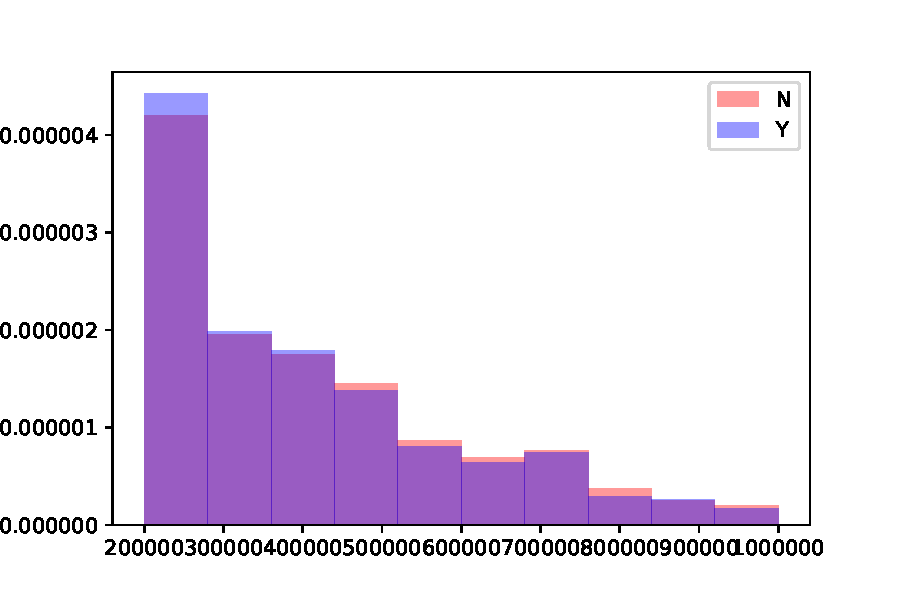
\includegraphics[width = \textwidth]{iznos_A.pdf}
			\caption[{\lstinline[language = Python, style = lijepo]{'A'}: Podjela po ugovorenom iznosu}]{\lstinline[language = Python, style = lijepo]{'A'}: Podjela po ugovorenom iznosu (između \ensuremath{2 \cdot 10^{5}} i \ensuremath{1 \cdot 10^{6}})}
		\end{subfigure}
		\hfill
		\begin{subfigure}{0.4\textwidth}
			\centering
			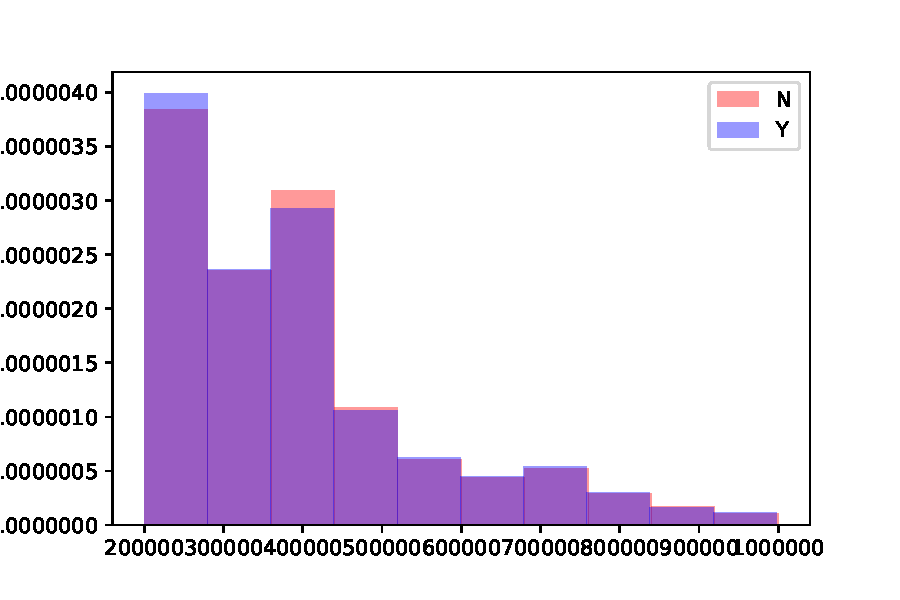
\includegraphics[width = \textwidth]{iznos_L.pdf}
			\caption[{\lstinline[language = Python, style = lijepo]{'L'}: Podjela po ugovorenom iznosu}]{\lstinline[language = Python, style = lijepo]{'L'}: Podjela po ugovorenom iznosu (između \ensuremath{2 \cdot 10^{5}} i \ensuremath{1 \cdot 10^{6}})}
		\end{subfigure}

		\par

		\begin{subfigure}{0.4\textwidth}
			\centering
			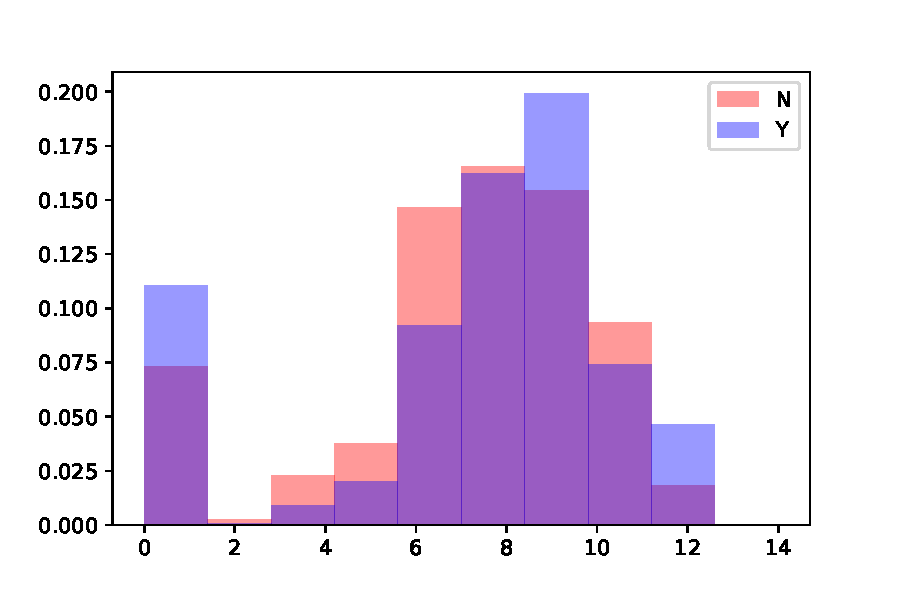
\includegraphics[width = \textwidth]{kamata_A.pdf}
			\caption[{\lstinline[language = Python, style = lijepo]{'A'}: Podjela po visini kamate}]{\lstinline[language = Python, style = lijepo]{'A'}: Podjela po visini kamate (do \ensuremath{14})}
		\end{subfigure}
		\hfill
		\begin{subfigure}{0.4\textwidth}
			\centering
			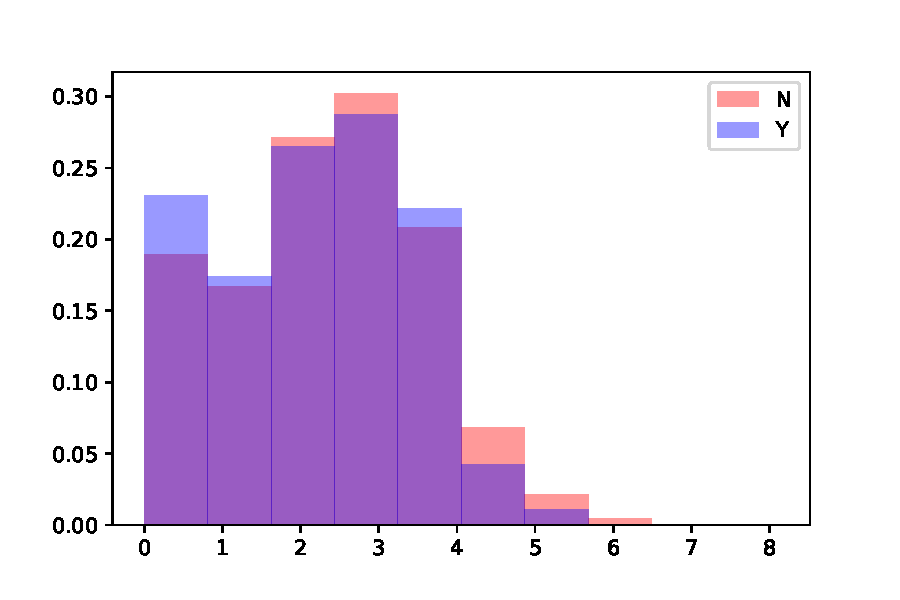
\includegraphics[width = \textwidth]{kamata_L.pdf}
			\caption[{\lstinline[language = Python, style = lijepo]{'L'}: Podjela po visini kamate}]{\lstinline[language = Python, style = lijepo]{'L'}: Podjela po visini kamate (do \ensuremath{8})}
		\end{subfigure}
		
		\par
		
		\begin{subfigure}{0.4\textwidth}
			\centering
			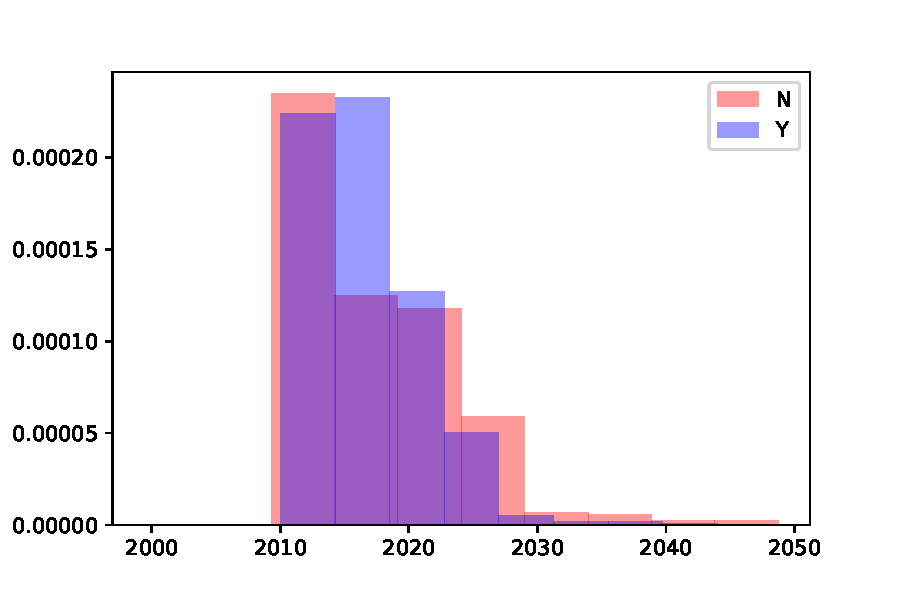
\includegraphics[width = \textwidth]{planirani_datum_zatvaranja_A.pdf}
			\caption{\lstinline[language = Python, style = lijepo]{'A'}: Podjela po planiranom datumu zatvaranja}
		\end{subfigure}
		\hfill
		\begin{subfigure}{0.4\textwidth}
			\centering
			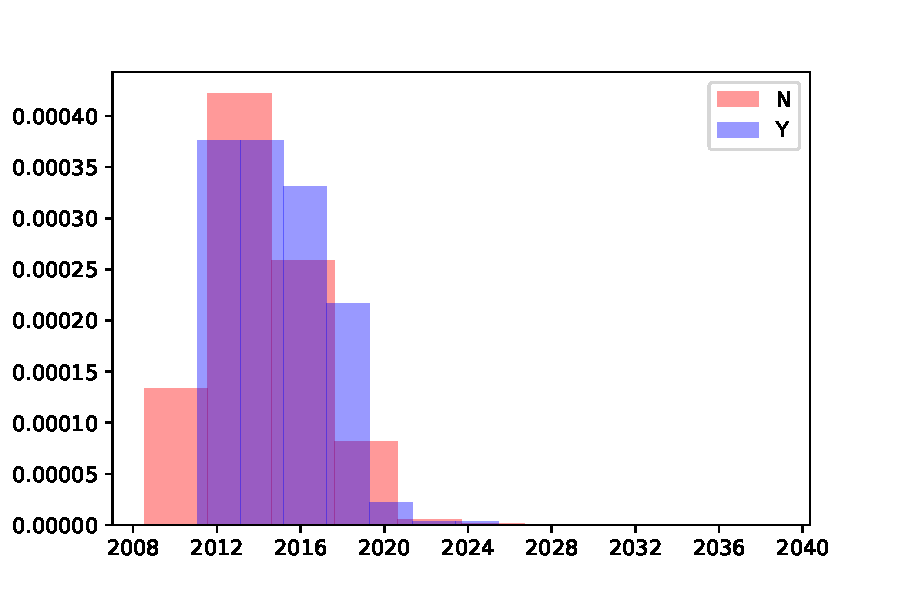
\includegraphics[width = \textwidth]{planirani_datum_zatvaranja_L.pdf}
			\caption{\lstinline[language = Python, style = lijepo]{'L'}: Podjela po planiranom datumu zatvaranja}
		\end{subfigure}
		
		\par
		
		\caption[Distribucije vrijednosti nekih značajki]{Distribucije vrijednosti nekih značajki po prijevremeno raskinutim i inim ugovorima, za svaku vrstu proizvoda posebno}
		\label{fig:histogrami}
	\end{figure}

	\par

	\section{Izvlačenje značajki i njihova značajnost u korištenom modelu}
	\label{sec:izvlacenje_znacajki}

	Dobiveni \emph{dataset} (treninški, evaluacijski i validacijski) prvo se \emph{spljošti} na način da se svi izvještaji o istom ugovoru (s istom oznakom partije) \emph{spljošte} u jedan redak. U tom su retku zapisane vremenski prva i zadnja vrijednost značajki koje mogu varirati (na primjer, ugovoreni iznos, kamata, datumi otvaranja i planiranog zatvaranja{\ldots}).

	\par

	Osim spljoštenja, izračunate su i neke značajke iz originalnog \emph{dataseta}, kao, na primjer, promjena ugovorenog iznosa, duljina planiranog trajanja ugovora, kamatni račun{\ldots} Nadalje, dodane su neke makroekonomske značajke (do datuma do kojeg postoje podatci ili predviđanja), poput prosjeka, standardne devijacije i trenda kretanja bruto domaćeg proizvoda u Republici Hrvatskoj ili cijene nafte. Konačno, dodane su neke značajke \emph{izmišljene} vlastitom logikom --- ocijene vjerojatnosti prijevremenog raskida po kombinacijama vrste klijenta, proizvoda i visine kamate izračunate statistički iz treninškog \emph{dataseta}, obuhvaćenost perioda trajanja ugovora u krizi i slično.

	\par

	Reinterpretacijom konstruiranih modela zaključuje se da su najbitnije značajke planirani datumi zatvaranja, planirana duljina trajanja ugovora i visina kamate. Kako su konstruirana $ 3 $ modela --- za ugovore vrste proizvoda \lstinline[language = Python, style = lijepo]{'A'} odnosno \lstinline[language = Python, style = lijepo]{'L'} planiranog datuma zatvaranja do $ 6 $. listopada $ 2016 $. godine i za ostale ugovore --- svaki, zapravo, ima vlastite značajnosti značajki, koje se mogu vidjeti pozivom metode \lstinline[language = Python, style = lijepo]{get_feature_importance} na odgovarajućem modelu.

	\par

	\section{Evaluirane metode}
	\label{sec:evaluirane_metode}

	Kao što je već spomenuto u dijelu~\ref{sec:izvlacenje_znacajki}, konstruirana su $ 3 $ modela. Za konstrukciju svakog od modela --- objekta klase \lstinline[language = Python, style = lijepo]{catboost.CatBoostClassifier} --- \href{http://hyperopt.github.io/hyperopt/}{paketom \emph{hyperopt}} izvršena je optimizacija hiperparametara modela, to jest, argumenata konstruktora. Optimizacija je vršena minimalizacijom razlike $ 1 $ i točnosti, preciznosti, odziva odnosno mjere $ F_{1} $ modela (zapravo, koristila se neka težinska sredina tih vrijednosti). Odabir hiperparametara koji se optimiziraju, kao i funkcije kojima se njihove vrijednosti biraju, rezultat je odluke autora rješenja nakon čitanja dokumentacije korištenih paketa, logičnog zaključivanja i više odnosno manje uspješnih pokušaja. Nakon optimizacije hiperparametara konačno je izvršen trening na više iteracija nego koliko se koristilo u testiranju pri optimizaciji hiperparametara.

	\par

	Baš zato što je ponašanje klijenata s ugovorima čiji se planirani datum zatvaranja ne će dogoditi unutar idućih nekoliko ili više godina, a konstruirani klasifikator mora predviđati trenutno stanje baze podataka banke \href{http://rba.hr/}{\emph{Reiffeisenbank Hrvatska}} (umjesto stanja za $ 10 $-$ 15 $ godina), ugovori čiji je planirani datum zatvaranja nakon $ 6 $. listopada $ 2016 $. godine klasificirani su kombinacijom modela za odgovarajuću vrstu proizvoda i modela za ugovore takvog kasnog planiranog datuma zatvaranja.

	\par

	Datum $ 6 $. listopada $ 2016 $. godine kao granica nije odabran arbitrarno. Autori ovog rješenja zaključili su da je to datum od godinu dana nakon završetka zadnje velike krize, do kojeg makroekonomski indikatori daju kompletnu sliku vanjskih utjecaja na ponašanje klijenata, a da kasniji planirani datumi zatvaranja (pogotovo oni nakon posljednjeg datuma izvještavanja koji je $ 31 $. prosinca $ 2018 $. godine) nisu predvidivi zbog manjka adekvatne ekonomske analize ili uopće ikakvih makroekonomskih podataka.

	\par

	\section{Analiza rješenja}
	\label{sec:analiza_rjesenja}

	Autori u svom rješenju pronalaze sljedeće vrline:
	\begin{enumerate}
		\item rješenje je interpretabilno --- iz modela se lako mogu \emph{ekstrahirati} značajke na temelju kojih se donosi odluka kao i njihovi udjeli u samoj klasifikaciji,
		\item rješenje generalizira problem --- iako je za konstrukciju rješenja \emph{dataset} fragmentiran na nekoliko dijelova, oni su još uvijek dovoljno veliki i općeniti da se iz njih može vidjeti logika zaključivanja, a fragmentacija modela opravdana je (v.\ dijelove \ref{sec:vizualizacija}, \ref{sec:izvlacenje_znacajki} i \ref{sec:evaluirane_metode}),
		\item rješenje je inovativno --- neke značajke izračunate su formulama koje su produkt razmišljanja autora rješenja, to jest, nisu neki općeniti ekonomski ili drugačiji indikatori kakvi se koriste u dosadašnjim modelima predikcije ponašanja klijenata, i autori smatraju da \href{http://catboost.ai}{paket \emph{CatBoost}} ne uživa popularnost (korištenost) kakvu zaslužuje.
	\end{enumerate}

	\par

	S druge strane, autori su svjesni i sljedećih mana rješenja:
	\begin{enumerate}
		\item na evaluacijskom \emph{datasetu} mjere kvalitete prediktora bile su niže od očekivanih,
		\item za treniranje modela korišten je veliki fond značajki od kojih neke možda na treninškom \emph{datasetu} slučajno imaju korelaciju s ciljnom varijablom, što se ne može lako detektirati pozivom metode \lstinline[language = Python, style = lijepo]{catboost.CatBoostClassifier} (s manjim fondom značajki ta bi detekcija možda bila lakša jer bi, idealno, dominirale one značajke koje imaju opravdanu i generalizirajuću korelaciju),
		\item neke su značajke međusobno inkonsistentno računate, a neke su računate nelogično ili čak pogrešno; neke pak ovise o poznatim vrijednostima makroekonomskih indikatora koji za predikciju budućnosti od nekoliko desetaka godina jednostavno ne postoje (ili postojeće predikcije donose veliku dozu nesigurnosti),
		\item model pretpostavlja poznavanje \emph{ponašanje} ugovora, to jest, je li se produljivao ili ne --- ovo nužno ne mora biti mana ako je dopušteno da u predikciju ponašanja klijenta za dani ugovor bude poznato je li taj ugovor već bio ranije ugovoren od istog klijenta s drugačijim stavkama.
	\end{enumerate}

	\par

	\addsec{Zaključak}

	S obzirom na dosadašnje znanje i iskustvo, kao i dostupna sredstva ((slobodno) vrijeme, računala, dostupnost podataka), autori su svojim rješenjem uglavnom zadovoljni. Ipak, preostaje dovoljno prostora za unaprjeđenje rješenja:
	\begin{enumerate}
		\item temeljitija analiza treninškog \emph{dataseta} --- zahtijeva više vremena i jače računalne kapacitete,
		\item pažljivija konstrukcija dodanih značajki --- nerijetko zahtijeva veću dostupnost (koja možda uopće nije moguća) vrijednosti: što dostupnih iz baze podataka banke (poput relevantne starosti klijenta, značenja vrijednosti značajki \emph{VRSTA\_KLIJENTA}, \emph{PROIZVOD}, {\emph{TIP\_KAMATE}}{\ldots}), što makroekonomskih pokazatelja,
		\item još temeljitija analiza mogućnosti \href{http://catboost.ai}{paketa \emph{CatBoost}}, kao i bolja optimizacija hiperparametara (možda i nekim drugim paketom osim \href{http://hyperopt.github.io/hyperopt/}{paketa \emph{hyperopt}}).
	\end{enumerate}
	Naime, različitim pokušajima, od kojih su svi vezani uz barem jednu od spomenutih točaka mogućeg daljnjeg unaprjeđenja rješenja, tijekom konstrukcije modela točnost klasifikacije rasla je, i to ponekad neočekivano velikim skokom. Autori smatraju da bi temeljitijim pristupom uvidjeli što je uspješnije pokušaje razlikovalo od neuspješnih pokušaja, čime bi se možda konstruirao zadovoljavajuće dobar model.

	\par

	Međutim, autori smatraju da ekstremno kvalitetni model primjenjiv u realnom poslovanju na ovakvom problemu nije moguće konstruirati, barem ne u timovima od $ 3 $ ili $ 4 $ studenta. Za predikciju ponašanja klijenta koji u današnje vrijeme ugovara kredit ili depozit na nekoliko desetaka godina jednostavno preostaje veliki broj nepoznatih vrijednosti koje bi vrlo vjerojatno \emph{domino-efektom} utjecale na to ponašanje. Za predviđanje tih parametara i konstrukciju modela koji je robustan na njihove greške, ako je takvo što uopće moguće, potreban je timski rad više stručnjaka iz različitih područja.

	\par
\end{document}
